% \chapter{Разработка собственного технического решения}
% \label{ch:chap3}

\section{Разработка принципиальной электрической схемы (или схемы соединений) вторичного преобразователя}
Принципиальная электрическая схема разрабатывается на основании анализа исходных данных и принятой функциональной схемы (рисунок \ref{fig:func_scheme}). Задача разработки электрической схемы проектируемого устройства заключается в выборе и обосновании принципиальных схем каскадов для реализации структурной схемы.

Вначале произведем анализ известных схемных решений проектируемого каскада. Критерии для разрабатываемой схемы: простота, надежность, дешевизна при выполнении заданных требований.

Исходя из разработанной функциональной схемы устройства принципиальная схема состоит из следующих функциональных узлов:
\begin{itemize}
    \item микроконтроллер (включает в себя АЦП);
    \item операционный усилитель;
    \item генератор высоких частот;
    \item блок питания;
    \item управляемый выпрямитель;
    \item RC-фильтр;
    \item емкостной датчик;
\end{itemize}

\newpage
\subsection{Микроконтроллер}
В качестве управляющего устройства выбран микроконтроллер ATmega8 (приложение \ref{appendmk}), использующийся в Arduino. Условное графическое обозначение микроконтроллера изображено
на рисунке \ref{fig:mk}.
\begin{figure}[ht]
	\centering
	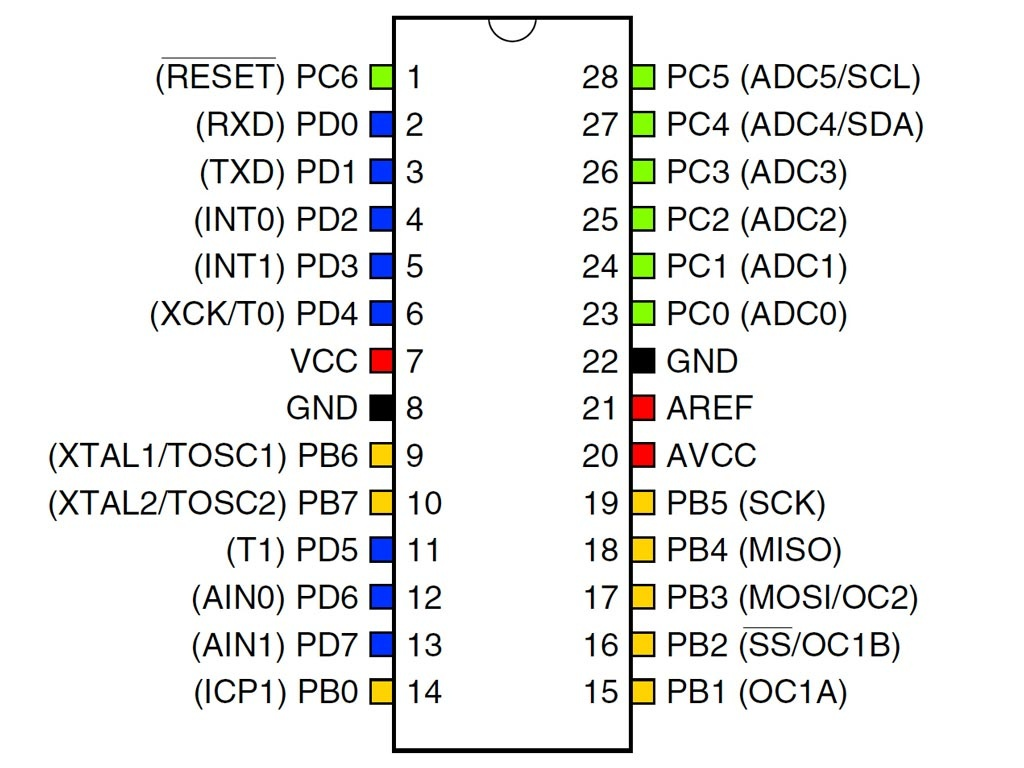
\includegraphics[width=0.6\textwidth]{./images/mk.png}
	\caption{Микроконтроллер ATmega8}
	\label{fig:mk}
\end{figure}
Характеристики:
\begin{itemize}
    \item Напряжение питания: 4.5…5.5 В;
    \item Ширина шины данных: 8-бит;
    \item Тактовая частота:	16 МГц;
    \item Количество входов/выходов: 23;
    \item Объем памяти программ: 8 кбайт;
    \item Тип памяти программ: flash;
    \item Встроенные интерфейсы: i2c, spi, uart;
    \item Напряжение питания: 4.5…5.5;
    \item Вес: 4 г;
    \item Наличие АЦП/ЦАП: да;
\end{itemize}
Микроконтроллер уже содержит в себе АЦП и может
давать на выход 16-битный параллельный код, а следовательно, не
требуется производить дополнительных преобразований выходного сигнала.


\subsection{Емкостной датчик}
Датчик собранный по схеме рисунка \ref{fig:sensor_scheme2}. Номиналы компонент датчика:
\(C_0 = 100\)пФ; \(C_d = 47\)пФ; \(L_k = 33\)мГн; \(R=510\)Ом.
Тогда контур обладает резонансной частотой 100КГц и добротностью 0.1. При напряжении питания генератора частот 15В ожидается уровень выходного сигнала порядка 1.5В.


\subsection{Операционный усилитель}
В схему требуется включить операционный усилитель, предназначенный для усиления аналогового сигнала. Выберем неинвертирующую схему усиления, поскольку в разрабатываемой принципиальной схеме отрицательные полуволны входного напряжения будут выпрямлены выпрямителем на входе схемы. Был выбран LM358 (приложение \ref{appendmult}).

\begin{figure}[ht]
	\centering
	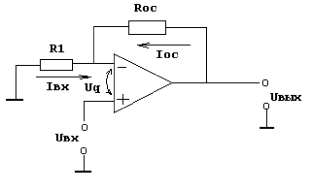
\includegraphics[width=0.6\textwidth]{./images/multiplier.png}
	\caption{Усилитель напряжения}
	\label{fig:multiplier}
\end{figure}
Коэффициент усиления представленной схемы рассчитывается по формуле \ref{eq:multiplier}.
\begin{equation}
    \label{eq:multiplier}
    \frac{U_{out}}{U_{in}} = \frac{R_{2} + R_1}{R_1} = 3
\end{equation}
Сигнал с датчика составляет порядка 1.5 В, а для работы микроконтроллера необходимо уровень от 2,6 до 5 В. 
Возьмем \(R_1 = 1\) кОм и \(R_2 = 2\) кОм, тогда коэффициент усиления равен~3.

\subsection{Генератор высоких частот}

В качестве генератора высоких частот был выбран EGP Proever XR2206 (приложение \ref{appendgenerator}). Требуемое питание 12 В, диапазон генерируемых частот 1Гц -- 1МГц. Обладает гибкой регулировкой, а так же несколькими режимами работы. Генератор будет работать с частотой 100 КГц, чтобы совпадать с резонансной частотой датчика.

\subsection{Блок питания}
Импульсный источник питания Mean Well RD-50A (приложение \ref{appendbp}). Блок питания с входным напряжением 220 В AC и выходными напряжениями 5 В DC (для МК) и 12 В DC (для ГВЧ), обеспечивающий стабильное питание компонентов устройства.

\subsection{RC-фильтр}
Длч фильтрации данных с датчика будем использовать RC-фильтр (рисунок \ref{fig:filter}). АЧХ такого фильтра беспрепятственно пропускает низкие частоты.
\begin{figure}[ht]
	\centering
	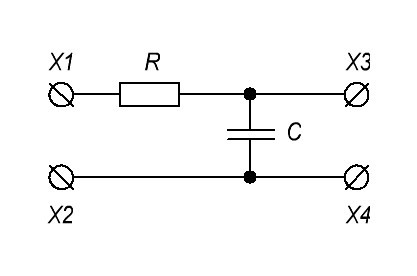
\includegraphics[width=0.6\textwidth]{./images/RC_filt.jpg}
	\caption{Схема RC-фильтра}
	\label{fig:filter}
\end{figure}
Частота среза рассчитывается по формуле
\begin{equation}
    \label{eq:filter}
    f_{c} = \frac{1}{2 \pi R_3 C_3}
\end{equation}
Частота среза должна быть 100кГц, потому что с такой частотой колеблется контур. В следствии этого были выбраны номиналы \(C_3 = 10\)нФ, \(R_3 = 1.6\)КОм.

\newpage
\section{Чертеж Э3 или Э4}
Чертеж представлен в СУИР.21.34352.001 Э3.
% \begin{figure}[ht]
% 	\centering
% 	\includegraphics[width=\textwidth]{./images/scheme.pdf}
% 	\caption{Схема подключения к МК: ИП -- источник питания; Д -- датчик; Z1 -- кварцевый ГВЧ; VD1...4 диоды; C1...C3 -- конденсаторы; R1...R4 -- резисторы; ОУ -- операционный усилитель;}
% 	\label{fig:pr_scheme}
% \end{figure}

На электрической схеме показан источник питания G1 подключен к сети AC 220В 50Гц и дает на выход два канала DC 5В и 12В.

Напряжение с 5В канала блока питания подается на микроконтроллер DD1. На базе элемента ZQ1 с конденсаторами С1 и С2 построен генератор тактовых сигналов. Он необходим для того, чтобы осуществлять работу микроконтроллера на постоянной частоте. Подключение осуществляется в порты XTAL1 и XTAL2 согласно схеме подключения выбранного микроконтроллера.

Напряжение с 12В канала блока питания подается на высокочастотный генератор DA1, который необходим для работы емкостного датчика. После этого сигнал с него идет на датчик DA2, выходом которого является напряжение порядка 1.5В, которое нам нужно измерить. Оно последовательно подается на диодный мост и RC-фильтр, состоящий из \(R_3\) и \(C_3\), после чего усиливается усилителем DA3 в 3 раза и подается на АЦП микроконтроллера PC5.

После этого микроконтроллер готов отдавать полученные значения в 16 битном формате. Для этого выделены порты [PD0...PD7] (старший байт), [PB0...PB5 PC0 PC1] (младший байт).
% , PC0 (синхронизация) и GND. 

Перечень элементов представлен в СУИР.21.34352.001 ПЭ3.
\endinput